\documentclass[conference, onecolumn]{IEEEtran}
\IEEEoverridecommandlockouts
\usepackage{graphicx}
\usepackage{textcomp}
\usepackage{xcolor}
\usepackage{subcaption}
\usepackage{float}

\begin{document}
\pagestyle{plain}

%----------------- Title Page -----------------
\begin{titlepage}

    \begin{center}
        
\includegraphics[width=0.5\textwidth]{figures/FPTU_logo.png}\\[1cm]

        {\LARGE \textbf{2025 Spring IOT102t Final Report}}\\[0.5cm]
        
        {\LARGE \textbf{IoT-based Weather Station}}\\[1cm]
        
        \textbf{Group Members:}\\
        Tran Dinh Son (SE184005)\\
        Truong Le Huy Hoang (SE192052)\\
        Nguyen Binh Minh (SE182173)\\
        Vo Nhat Thien (SE182141)\\
        
        \textbf{Supervisor}: Duc Ngoc Minh Dang\\[0.5cm]
        
        \textbf{FPT University, Ho Chi Minh Campus}\\
        
        \textbf{sontdse184005@fpt.edu.vn, minhnbse182173@fpt.edu.vn,}\\
        \textbf{thienvonhat@gmail.com, hoanghuypeter1182004@gmail.com,}\\
        \textbf{and ducdnm2@fe.edu.vn}\\[2cm]
        
    \end{center}

%----------------- Abstract -----------------
\begin{abstract}
This work explains the design, development, and evaluation of an IoT-based weather station for real-time observation of environmental factors such as temperature, humidity, atmospheric pressure, and rain. Using a set of onboard sensors interfaced to an ESP8266 microcontroller, the system offers wireless data transmission to a central server for remote analysis and visualization. The project presents a comprehensive approach covering hardware and
software modules including interfacing of sensors, processing algorithms for data, and a simple graphical interface. The highest priority is placed on the system adapting to various conditions in the environment, ensuring scalability and reliability. Experimental outcomes verify the monitoring system's efficacy and accuracy and, therefore, establish its applicability in smart city initiatives, precision agriculture, and disaster relief management. System step-by-step models, block diagrams, and program flowcharts
more effectively illustrate the technical underpinnings and development process. This report emphasizes the importance of integrating IoT technologies into meteorological use, providing the potential for innovative solutions in environmental monitoring and data-based decision making.

\end{abstract}

\end{titlepage}

%----------------- Table of Contents -----------------
\newpage
\tableofcontents
\newpage
    

%----------------- Section I: Introduction -----------------
\section{INTRODUCTION}
In recent years, IoT-based weather stations have emerged as important tools for environmental monitoring and real-time data acquisition. However, the installation and long-term maintenance of such systems are restricted by a series of technical and operational challenges that are applicable both locally and on a global scale.

On a local scale, research efforts are directed primarily towards the development of low-cost methods for sensor calibration and maintenance. The age-old issue of sensor drift necessitates the exploration of new calibration techniques to ensure the long-term accuracy and reliability of measurements, particularly under resource-constrained conditions. In addition, the limitations of existing communication infrastructures in rural or remote areas pose tremendous challenges to continuous data transmission.

Globally, IoT-based weather stations are becoming more advanced due to improved sensor technology and modern communication protocols such as LoRaWAN and NB-IoT. Researchers are working to integrate these standards into smart city networks, making data exchange more efficient and ensuring that different systems can easily work together through standardized data formats. At the same time, energy-efficient designs and energy harvesting methods are being emphasized for remote deployments, while robust security measures are needed to protect against cyber attacks. 

Lastly, ensuring that these systems are durable in extreme weather conditions remains a key priority. The dual concerns of environmental flexibility and system resilience stress the need for systems design approaches embracing technological innovation across the hardware, software, and network domains.

\vspace{10pt}
\noindent\rule{\textwidth}{0.4pt}
\vspace{10pt}

%----------------- Section II: Main Proposal -----------------
\section{MAIN PROPOSAL}
\subsection{System Models and Block Diagram}
The weather station consists of multiple sensors for environmental data collection, a microcontroller for data processing, and wireless communication modules for data transmission.

\begin{figure}[H]
    \centering
    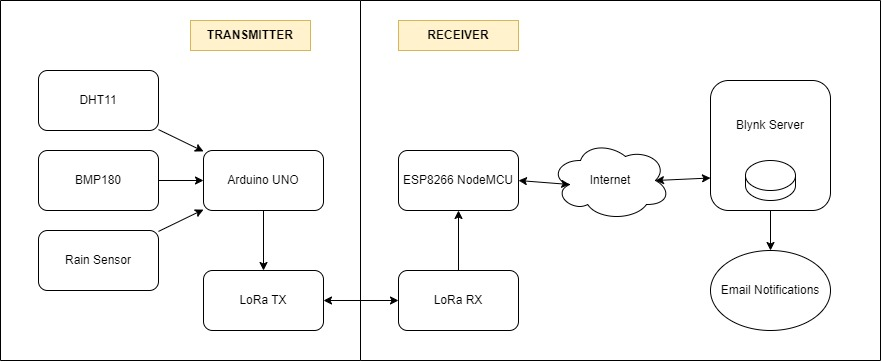
\includegraphics[width=0.5\textwidth]{figures/Weather_Station-Block_Diagram.jpg}
    \caption{Block Diagram of Weather Station}
    \label{fig:block_diagram}
\end{figure}

\textbf{System Model:}
\begin{itemize}
    \item \textbf{Data Collection:} Sensors (DHT11, BMP180, Rain Sensor) measure temperature, humidity, pressure, and rainfall.
    \item \textbf{Data Processing:} Arduino UNO R3 processes sensor readings and formats them for transmission.
    \item \textbf{Data Transmission:} LoRa RF433 SX1278 sends data to a receiver connected to the cloud via ESP8266 NodeMCU.
    \item \textbf{Data Visualization:} The Blynk server stores and displays real-time weather data for remote access, as well as alerts users about extreme weather (heavy rainfall, high temperature, etc.) via mobile app and Gmail
\end{itemize}

\begin{figure}[H]
    \centering
    \begin{subfigure}{0.45\textwidth}
        \centering
        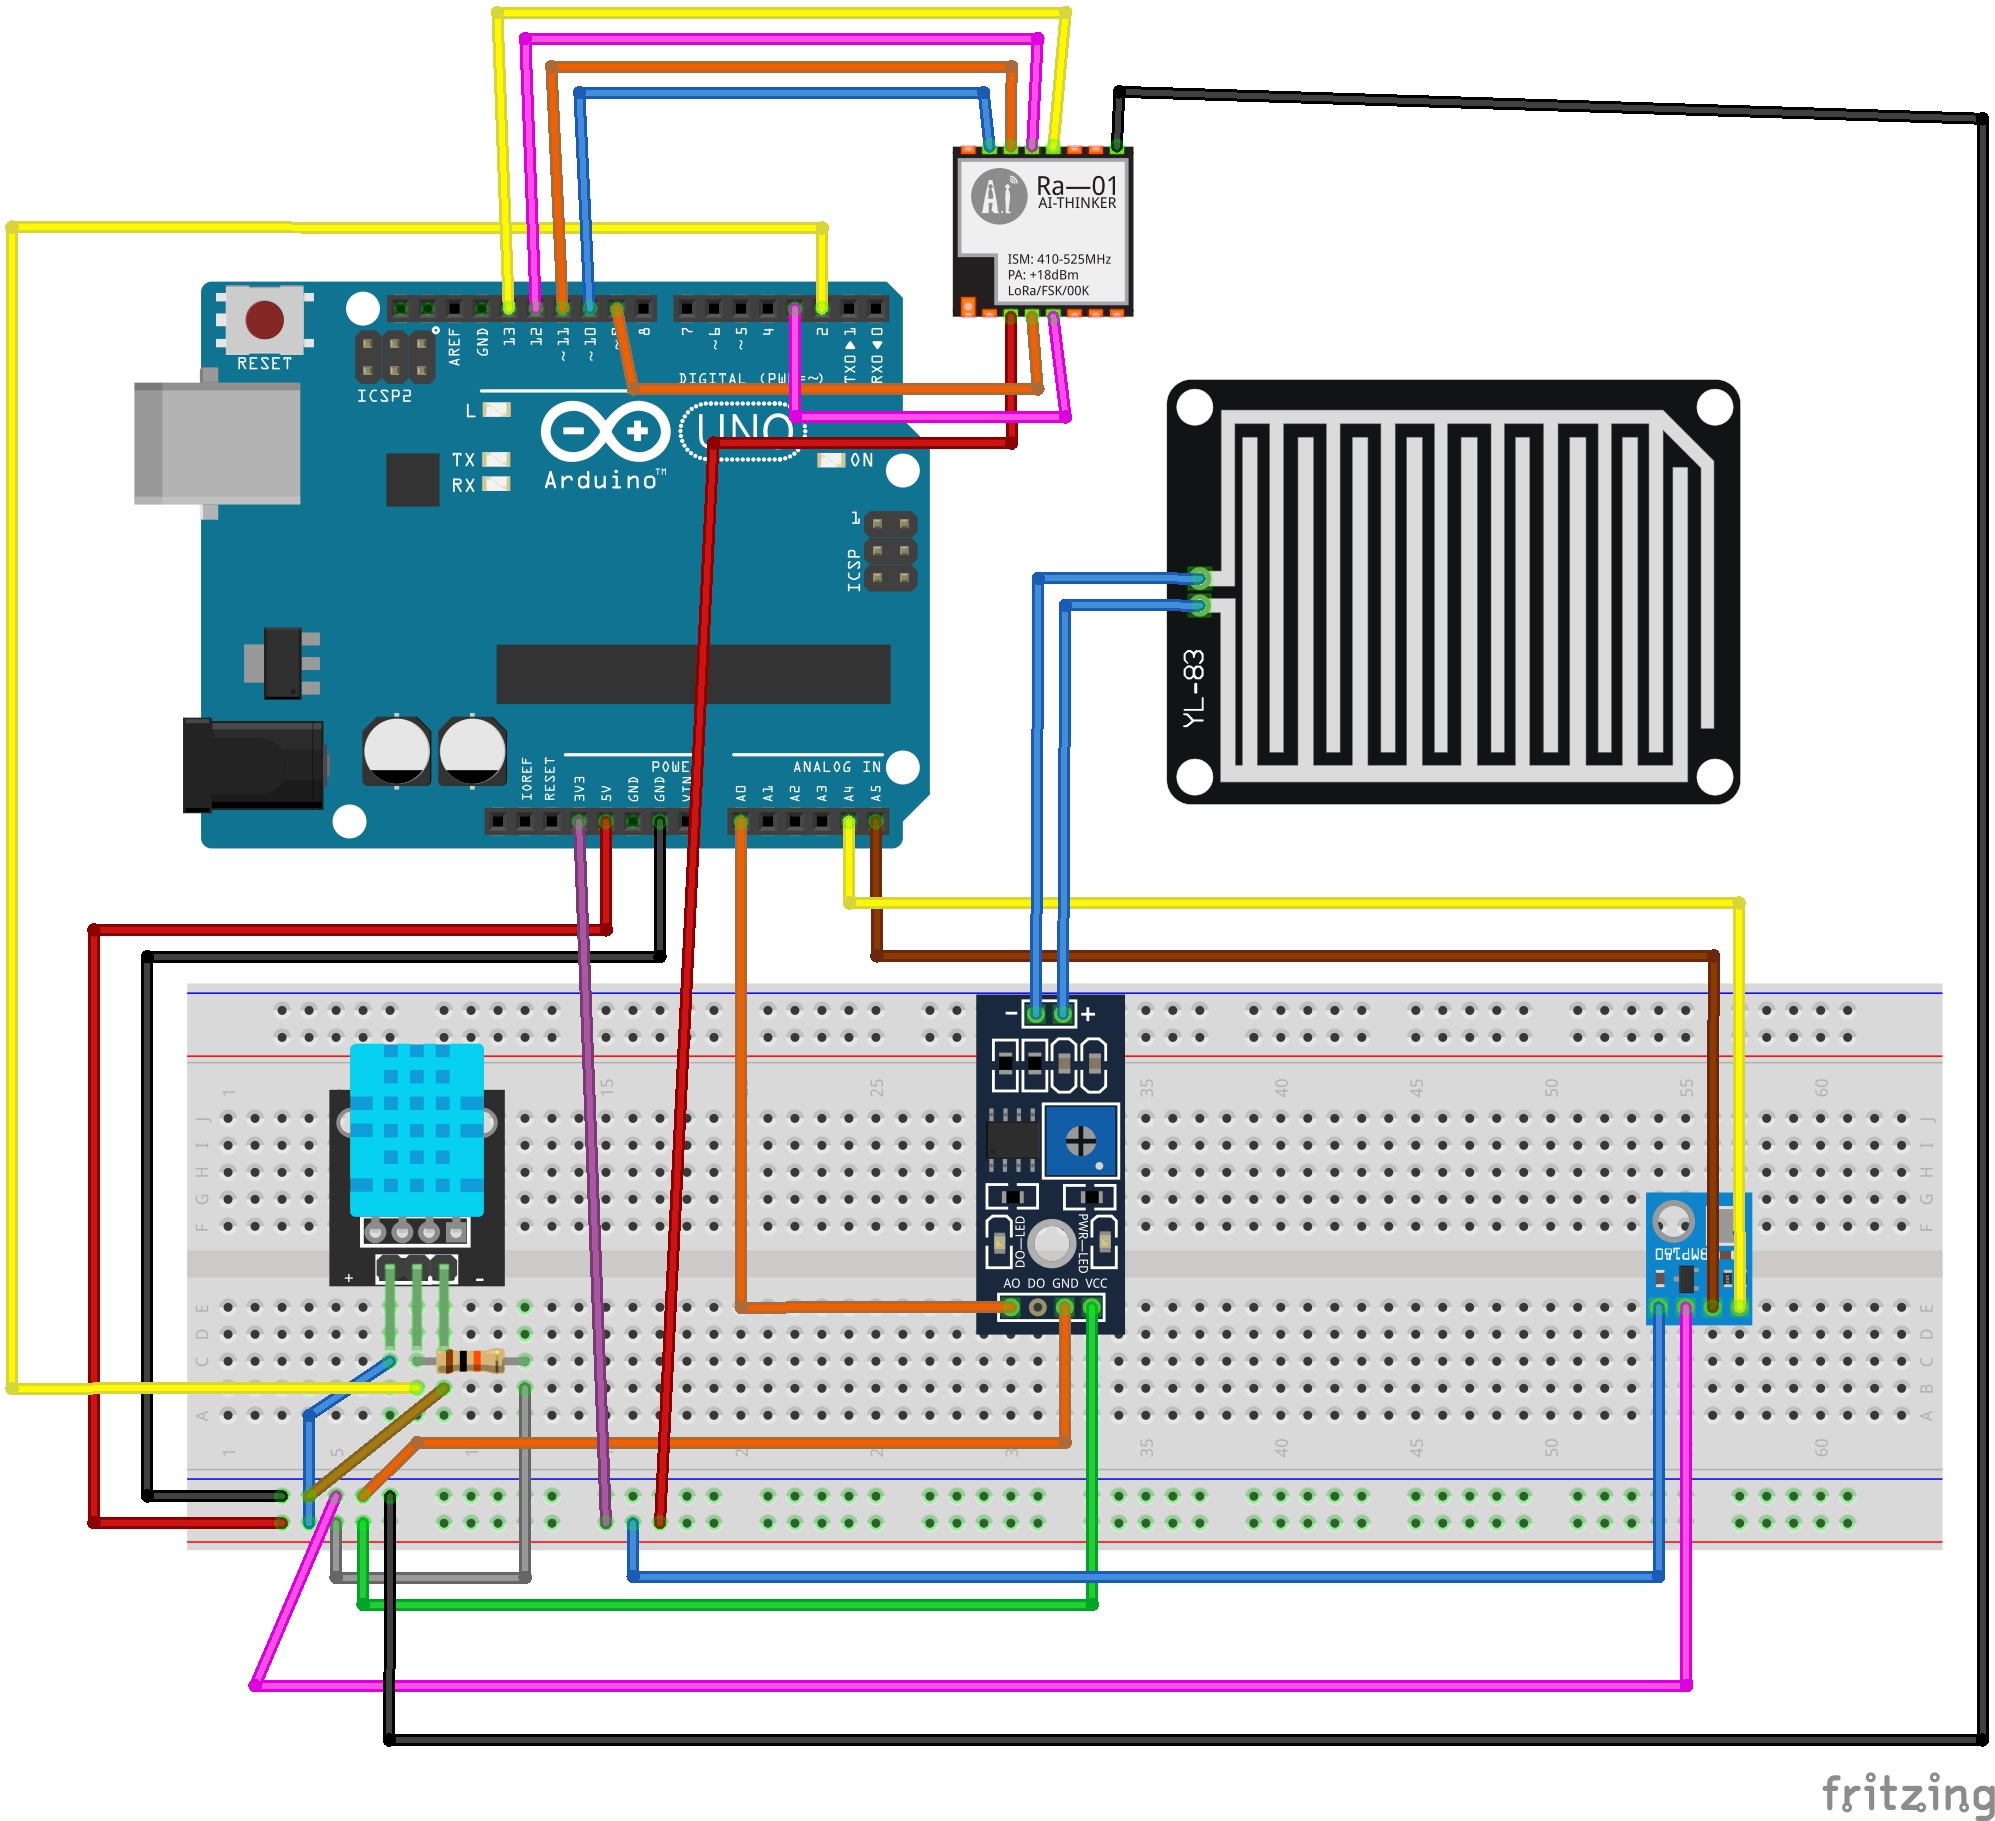
\includegraphics[width=0.535\linewidth]{figures/Weather_Station_Arduino.jpg}
        \caption{Arduino UNO with LoRa}
        \label{fig:esp8266_lora}
    \end{subfigure}
    \hfill
    \begin{subfigure}{0.45\textwidth}
        \centering
        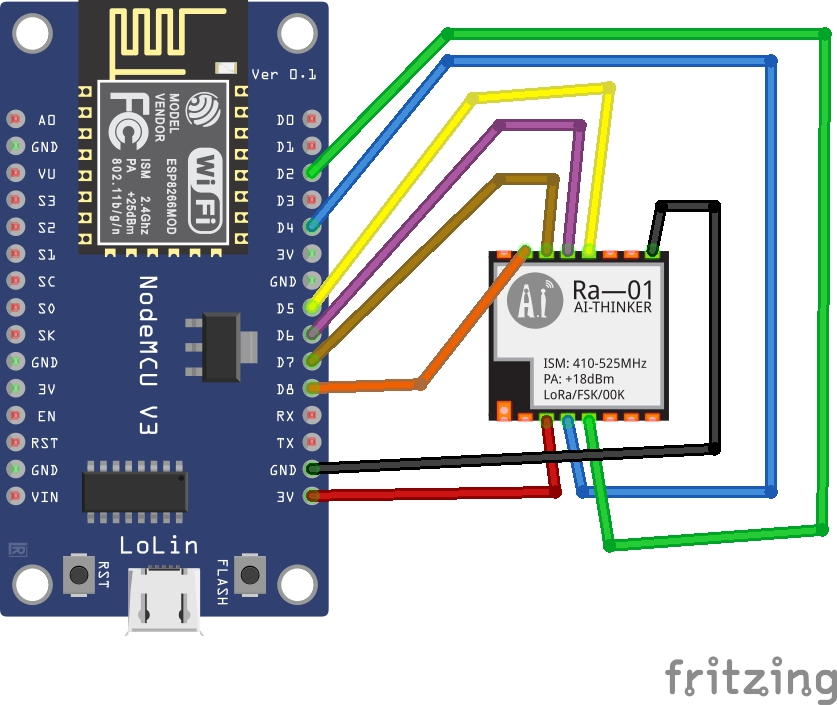
\includegraphics[width=0.535\linewidth]{figures/Weather_Station_ESP.jpg}
        \caption{ESP8266 NodeMCU with Sensors}
        \label{fig:arduino_sensors}
    \end{subfigure}
    \caption{Circuit Diagram for Weather Station System}
    \label{fig:weather_station}
\end{figure}

\subsection{Components and Peripheral Devices}
\begin{itemize}
    \item \textbf{Microcontroller:} Arduino UNO R3 ATMEGA16U2 – Processes sensor data and controls system functions.
    \item \textbf{Sensors:}
    \begin{itemize}
        \item DHT11: Measures temperature and humidity.
        \item BMP180: Monitors atmospheric pressure.
        \item Rain sensor: Detects the intensity of the rain.
    \end{itemize}
    \item \textbf{Wireless Communication Modules:}
    \begin{itemize}
        \item LoRa RF433 SX1278 Modules: Transmit sensor data over long distances.
        \item ESP8266 NodeMCU: Connects to WiFi for cloud-based monitoring.
    \end{itemize}
    \item \textbf{Display \& Indicators:}
    \begin{itemize}
        \item Blynk App: Provides real-time weather updates on a smartphone.
        \item Gmail / Blynk app: Alerts users to extreme weather conditions.
    \end{itemize}
\end{itemize}

\begin{figure}[H]
    \centering
    \begin{subfigure}{0.45\textwidth}
        \centering
        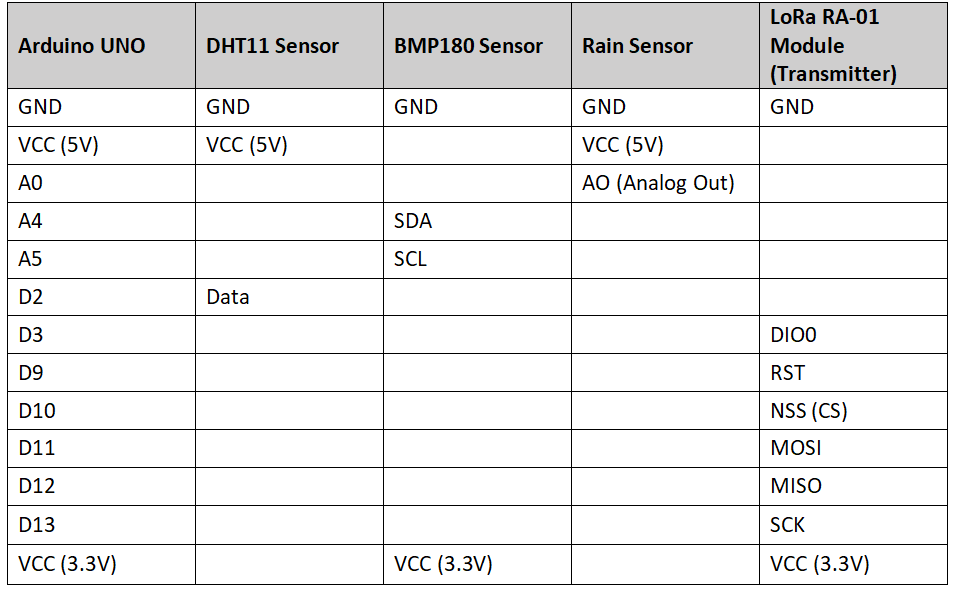
\includegraphics[width=\linewidth]{figures/Screenshot 2025-03-01 154513.png}
        \caption{Arduino UNO Interfacing}
        \label{fig:arduino_interfacing}
    \end{subfigure}
    \hfill
    \begin{subfigure}{0.45\textwidth}
        \centering
        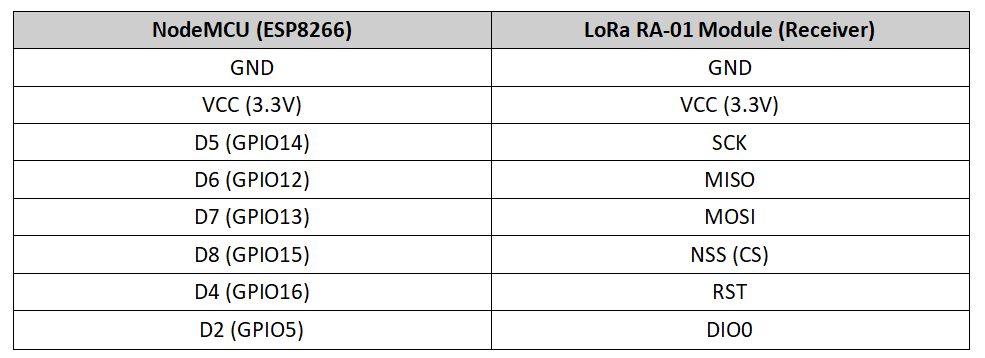
\includegraphics[width=\linewidth]{figures/Screenshot 2025-03-01 154646.png}
        \caption{ESP8266 NodeMCU Interfacing}
        \label{fig:esp8266_interfacing}
    \end{subfigure}
    \caption{Hardware Interfacing for Weather Station System}
    \label{fig:weather_station_interfacing}
\end{figure}

\subsection{Software Programming}
The system is programmed using Arduino IDE with C/C++ for microcontroller control. The software structure includes the following:
\begin{itemize}
    \item \textbf{Sensor Data Acquisition:} Reads data from DHT11, BMP180, and Rain Sensor at regular intervals.
    \item \textbf{Data Processing:} Filters and formats sensor readings.
    \item \textbf{Wireless Communication:}
    \begin{itemize}
        \item LoRa transmits data from the remote station to a central receiver.
        \item ESP8266 connects to the Blynk server for cloud visualization.
    \end{itemize}
    \item \textbf{Alerts and Notifications:} Threshold-based alerts for abnormal weather conditions.
    \item \textbf{Real-time Data Logging:} Blynk server stores historical weather data for analysis.
\end{itemize}

\subsection{Programming Flowchart}
\begin{enumerate}
    \item Start
    \item Initialize System Components
    \begin{itemize}
        \item Initialize Serial Communication
        \item Initialize Sensors (DHT11, BMP180, Rain Sensor)
        \item Initialize Communication Modules (LoRa, ESP8266)
        \item Verify Initialization Success (Print Errors if Failed)
    \end{itemize}
    \item Transmitter Side Processing (Arduino)
    \begin{itemize}
        \item Run Blynk
        \item Read Data from Sensors (DHT11, BMP180, Rain Sensor)
        \item Check for Sensor Connection Errors (Print Errors if Failed)
        \item Process and Parse Sensor Data
        \item Transmit Data via LoRa to Receiver
    \end{itemize}
    \item Receiver Side Processing (ESP8266)
    \begin{itemize}
        \item Check for Incoming LoRa Packets (Print Errors if Not Received)
        \item Read and Parse Received Data
        \item Send Processed Data to Blynk for Cloud Storage
    \end{itemize}
    \item Threshold Monitoring \& Alerts
    \begin{itemize}
        \item Compare Sensor Data with Defined Thresholds
        \item If exceeded → Trigger alerts via mobile app and email notifications
        \item If within range → Continue Monitoring
    \end{itemize}
    \item Repeat Process (Loop Back to Step 3)
\end{enumerate}

\begin{figure}[H]
    \centering
    \begin{subfigure}{0.45\textwidth}
        \centering
        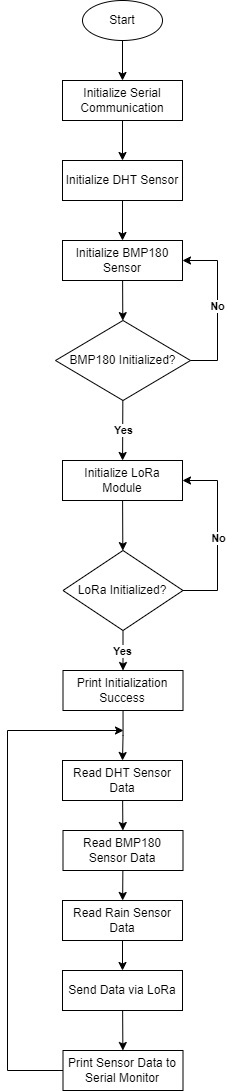
\includegraphics[width=0.45\linewidth]{figures/Weather_Station-Arduino_Flowchart.jpg}
        \caption{Arduino Flowchart}
        \label{fig:arduino_flowchart}
    \end{subfigure}
    \hfill
    \begin{subfigure}{0.45\textwidth}
        \centering
        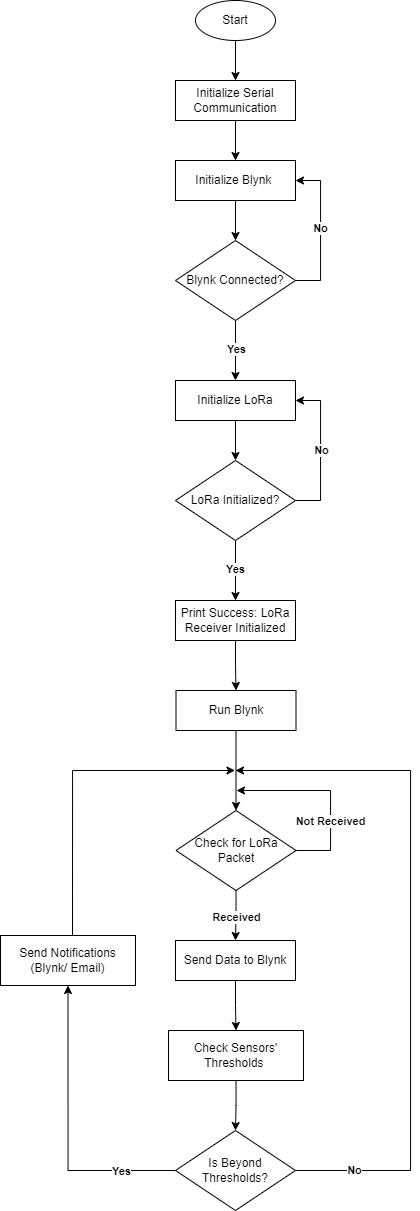
\includegraphics[width=0.72\linewidth]{figures/Weather_Station-ESP8266_Flowchart.jpg}
        \caption{ESP8266 Flowchart}
        \label{fig:esp8266_flowchart}
    \end{subfigure}
    \caption{Flowcharts for Weather Station System}
    \label{fig:weather_station_flowchart}
\end{figure}

\vspace{10pt}
\noindent\rule{\textwidth}{0.4pt}
\vspace{10pt}

%----------------- Section III: Results and Discussion -----------------
\section{RESULTS AND DISCUSSION}
The research methodology employed within this project involved the utilization of calibrated sensors to collect environment data in the field, after which wireless transmission was facilitated using protocols like LoRa and WiFi. The data were monitored real-time continuously with alarm systems that were automated to instantly determine and correct anomalies. Testing was iterative so as to guarantee sensor precision, test connectivity, and data integrity throughout collection, transmission, and storage.

\subsection{Prototype Implementation}
The prototype development involved several key steps. First, the hardware installation integrated sensors, microcontrollers (Arduino and NodeMCU), and LoRa modules to form the physical basis of the system. Subsequently, software development was undertaken to program sensor data collection, wireless communication, and real-time monitoring via Blynk. Extensive testing and debugging were performed to validate sensor accuracy, reliable connectivity, and system stability in general. The software and hardware components were then merged and optimized to deliver maximum performance. Finally, the ultimate system was demonstrated and tested to confirm that it meets the intended objectives.

\subsection{Experimental Results}

\begin{figure}[H]
    \centering
    \begin{subfigure}{0.45\textwidth}
        \centering
        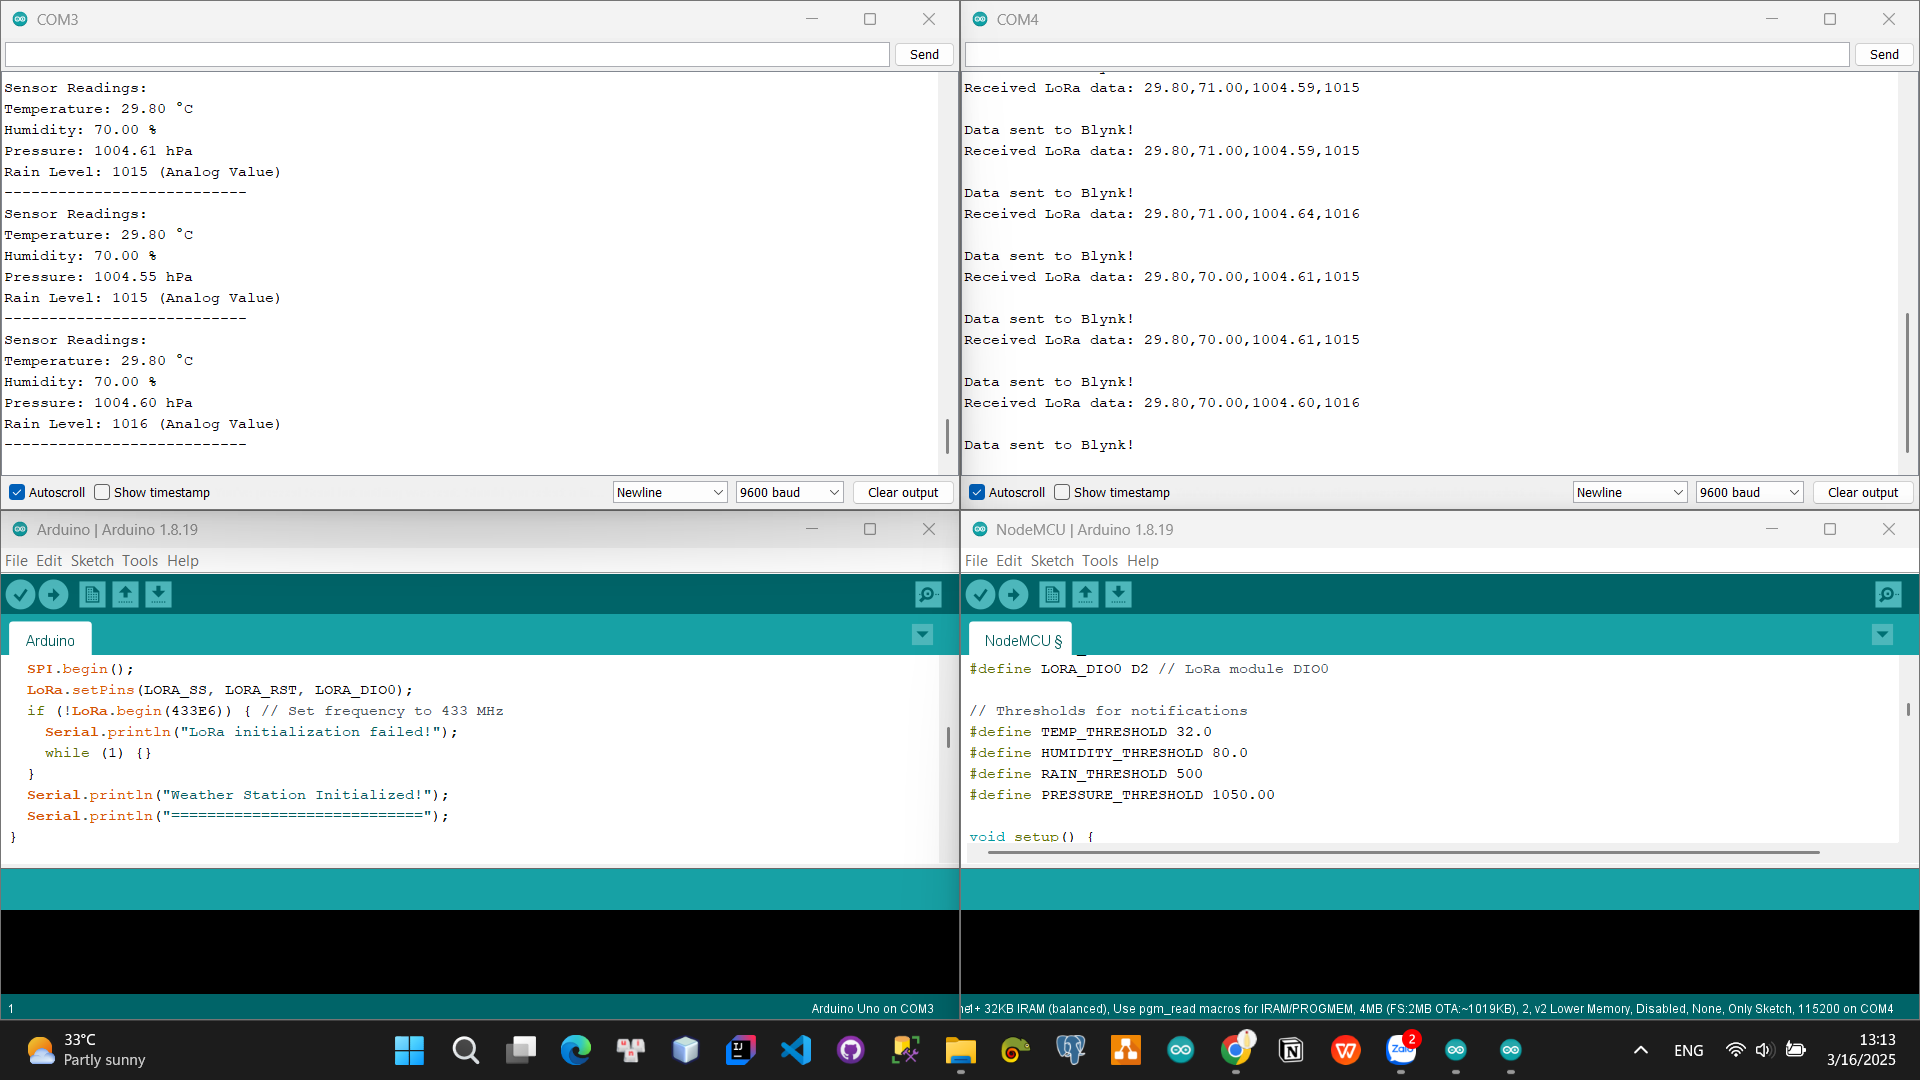
\includegraphics[width=0.9\linewidth]{figures/Screenshot (197).png}
        \caption{Serial Monitor on Arduino and ESP8266} 
        \label{fig:serial_monitor}
    \end{subfigure}
    \hfill
    \begin{subfigure}{0.45\textwidth}
        \centering
        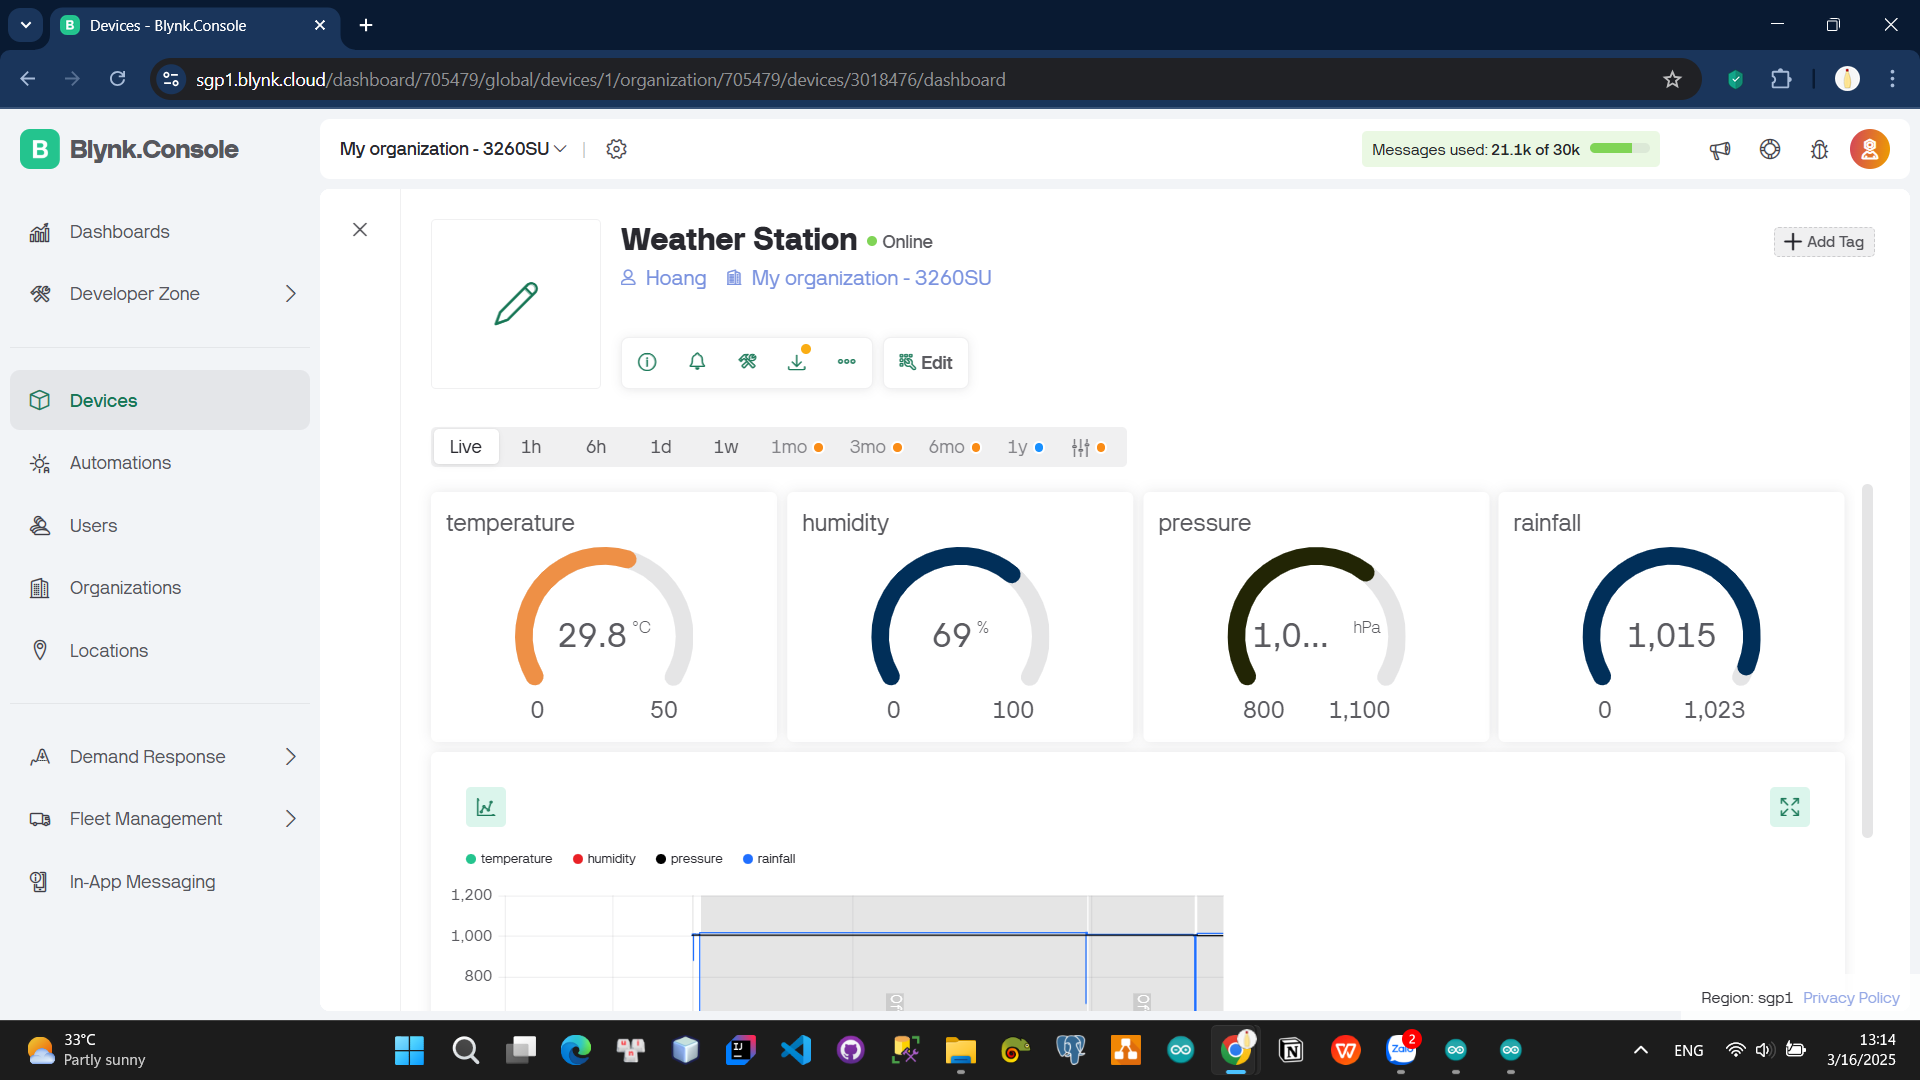
\includegraphics[width=0.9\linewidth]{figures/Screenshot (199).png}
        \caption{Blynk Console showing real-time weather station data}
        \label{fig:blynk_console}
    \end{subfigure}
    \caption{Real-time data results displayed on the Serial Monitor and the Blynk Console}
    \label{fig:data_results}
\end{figure}

During the experimental setup, sensor readings were collected and transmitted wirelessly to a server platform for centralized monitoring. Collected data were processed for validity and authenticity against expected environmental values. Periods of data transmission and potential offline intervals are also visible.

\begin{figure}[H]
    \centering
    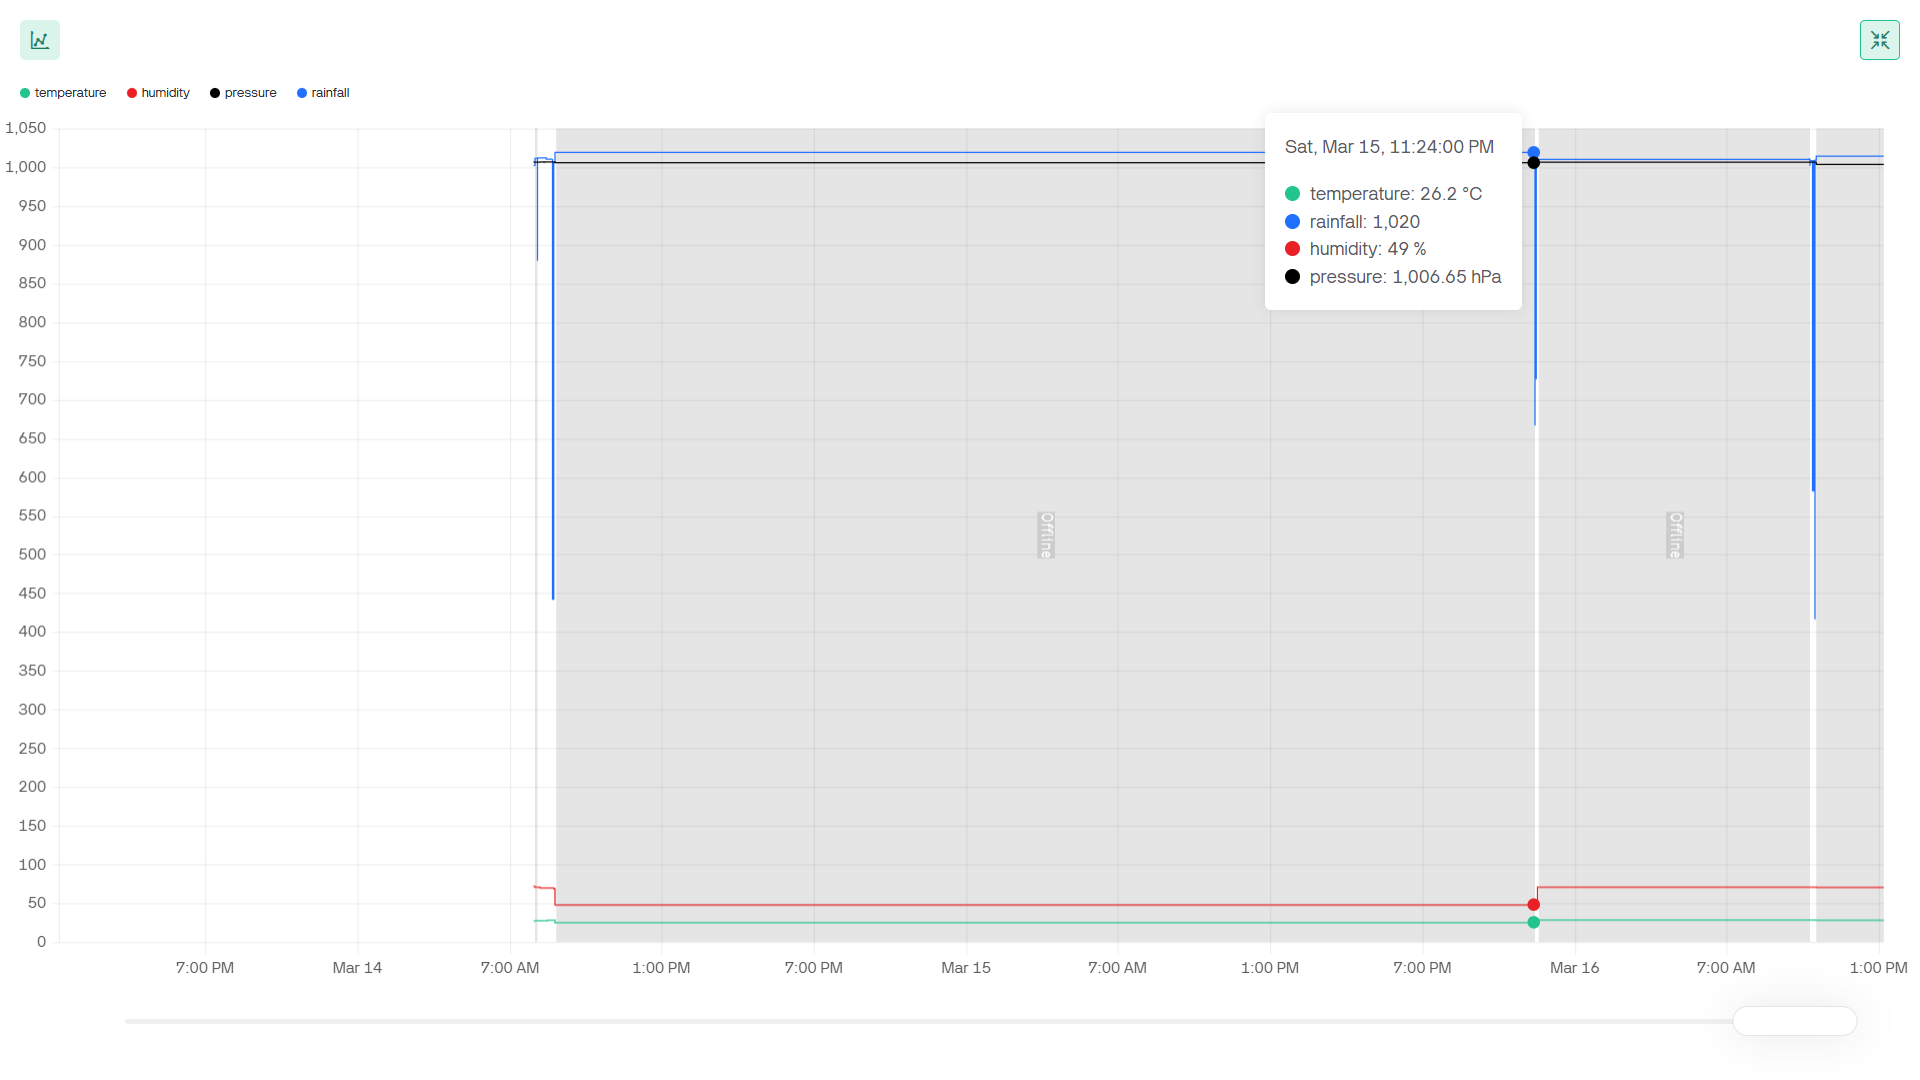
\includegraphics[width=0.7\textwidth]{figures/Screenshot (200).png}
    \caption{Weather Station Data Visualization on Blynk Dashboard}
    \label{fig:collected_data}
\end{figure}

In the results, it was discovered that real-time monitoring of the system is feasible, and threshold-based alerts are triggered through mobile notification and email for high-temperature, humidity, rain, and pressure parameters. It highlights the effectiveness as well as the limitations of current implementation.

\begin{figure}[H]
    \centering
    \begin{subfigure}{0.45\textwidth}
        \centering
        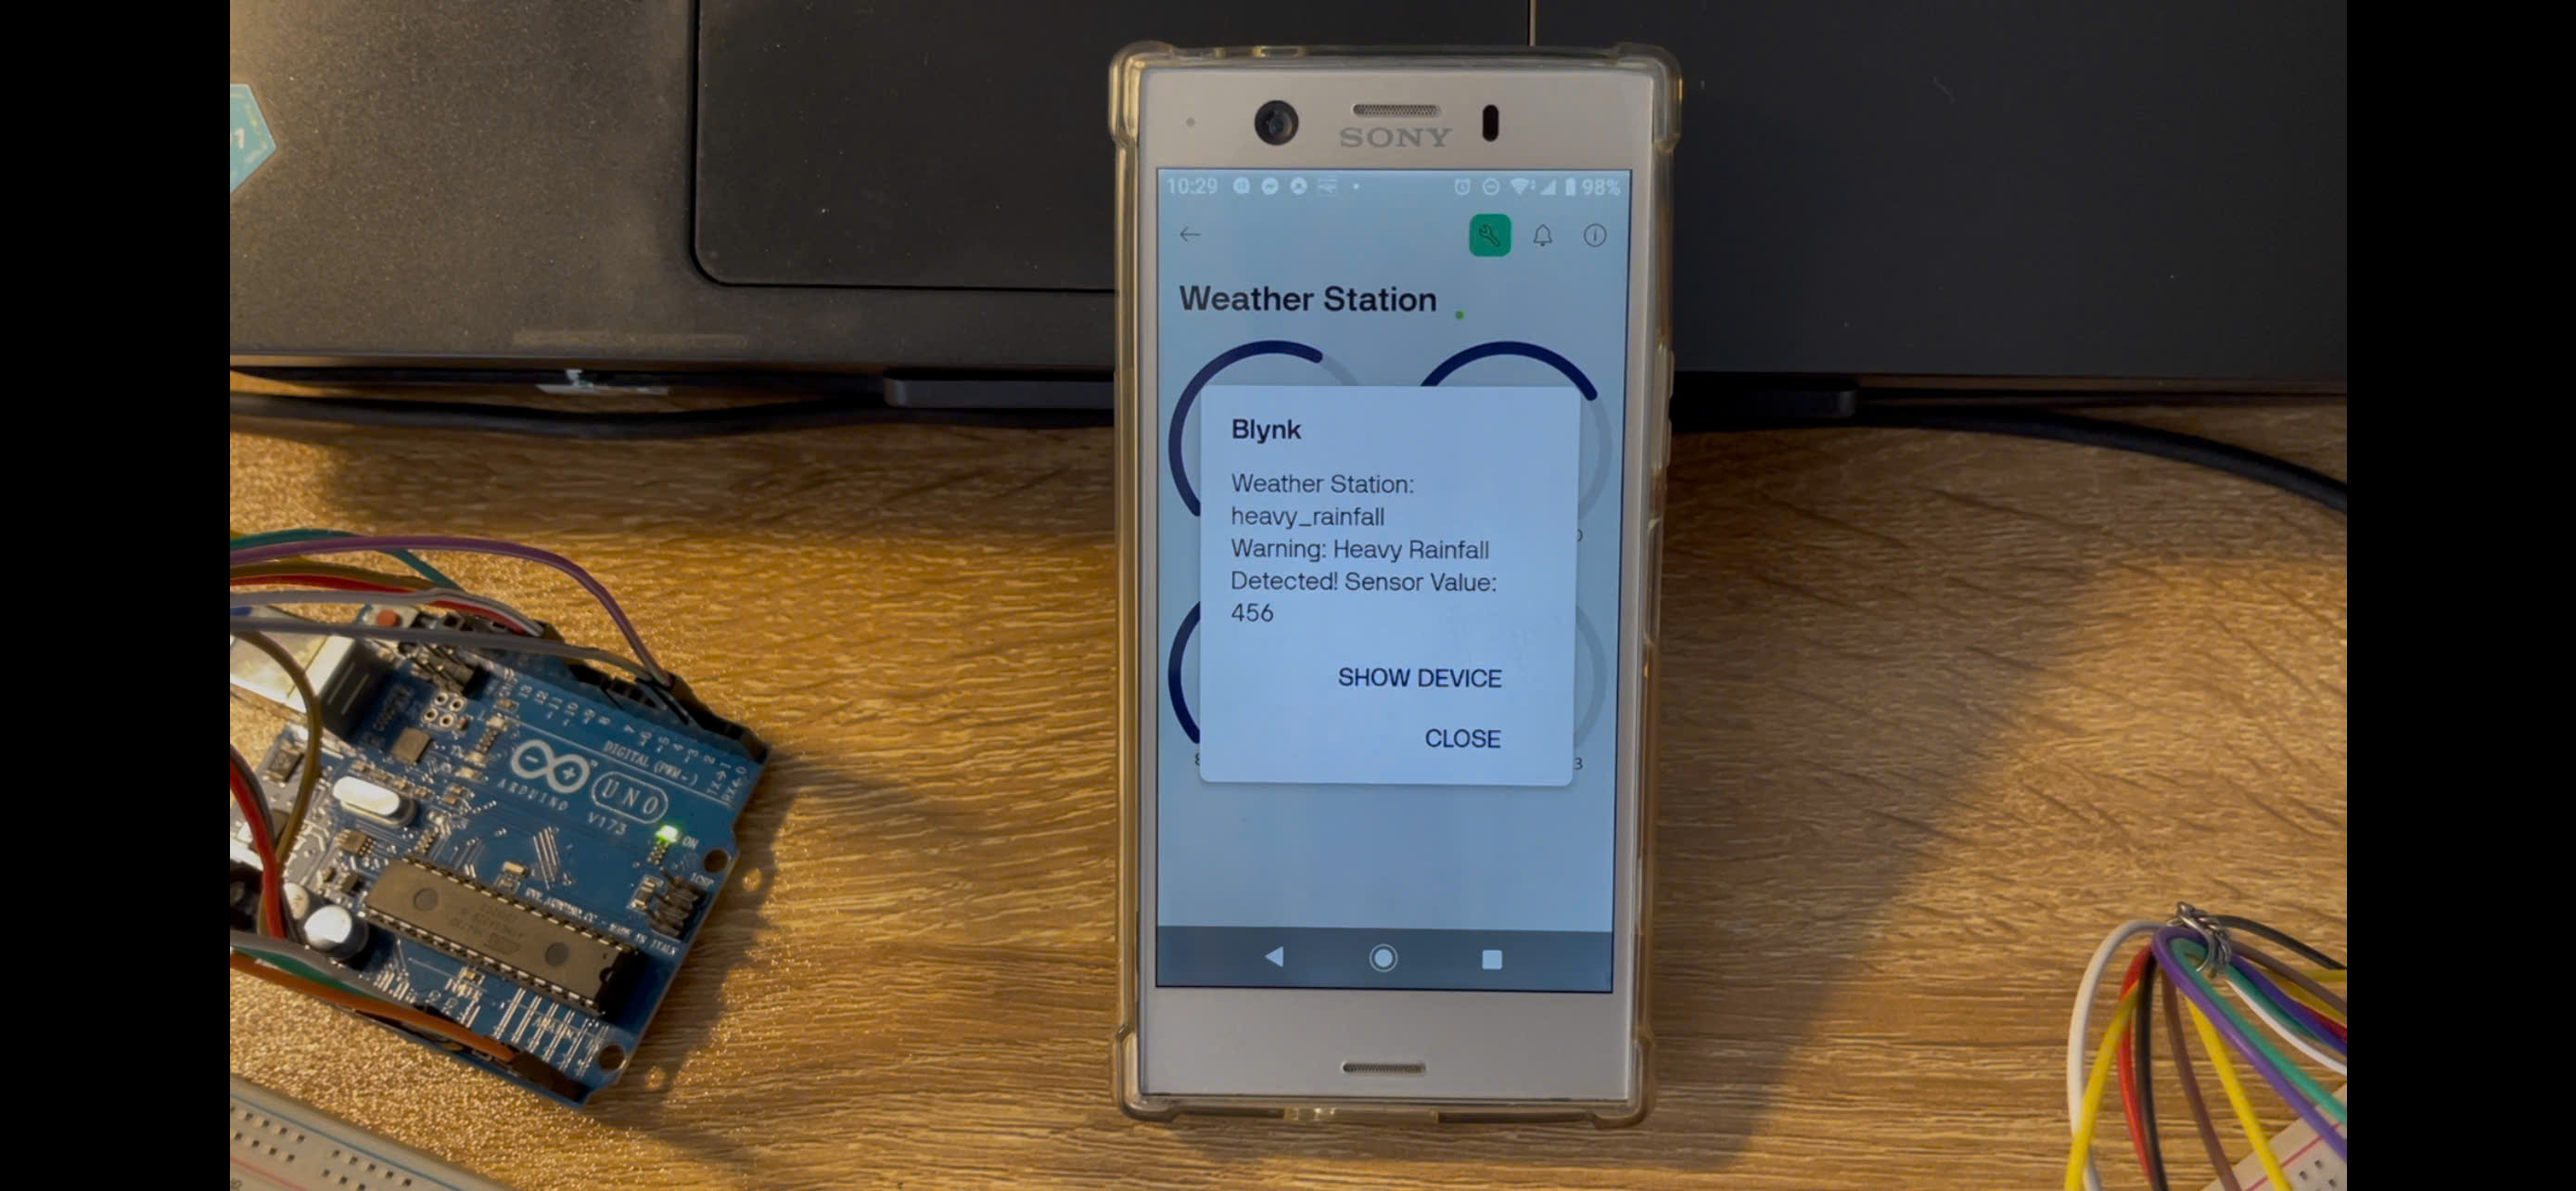
\includegraphics[width=0.9\linewidth]{figures/z6411778617685_cbd16394e12ac6a735b409c7785fee52.jpg}
        \caption{Alerts on Blynk Mobile App} 
        \label{fig:mobile_app_alerts}
    \end{subfigure}
    \hfill
    \begin{subfigure}{0.45\textwidth}
        \centering
        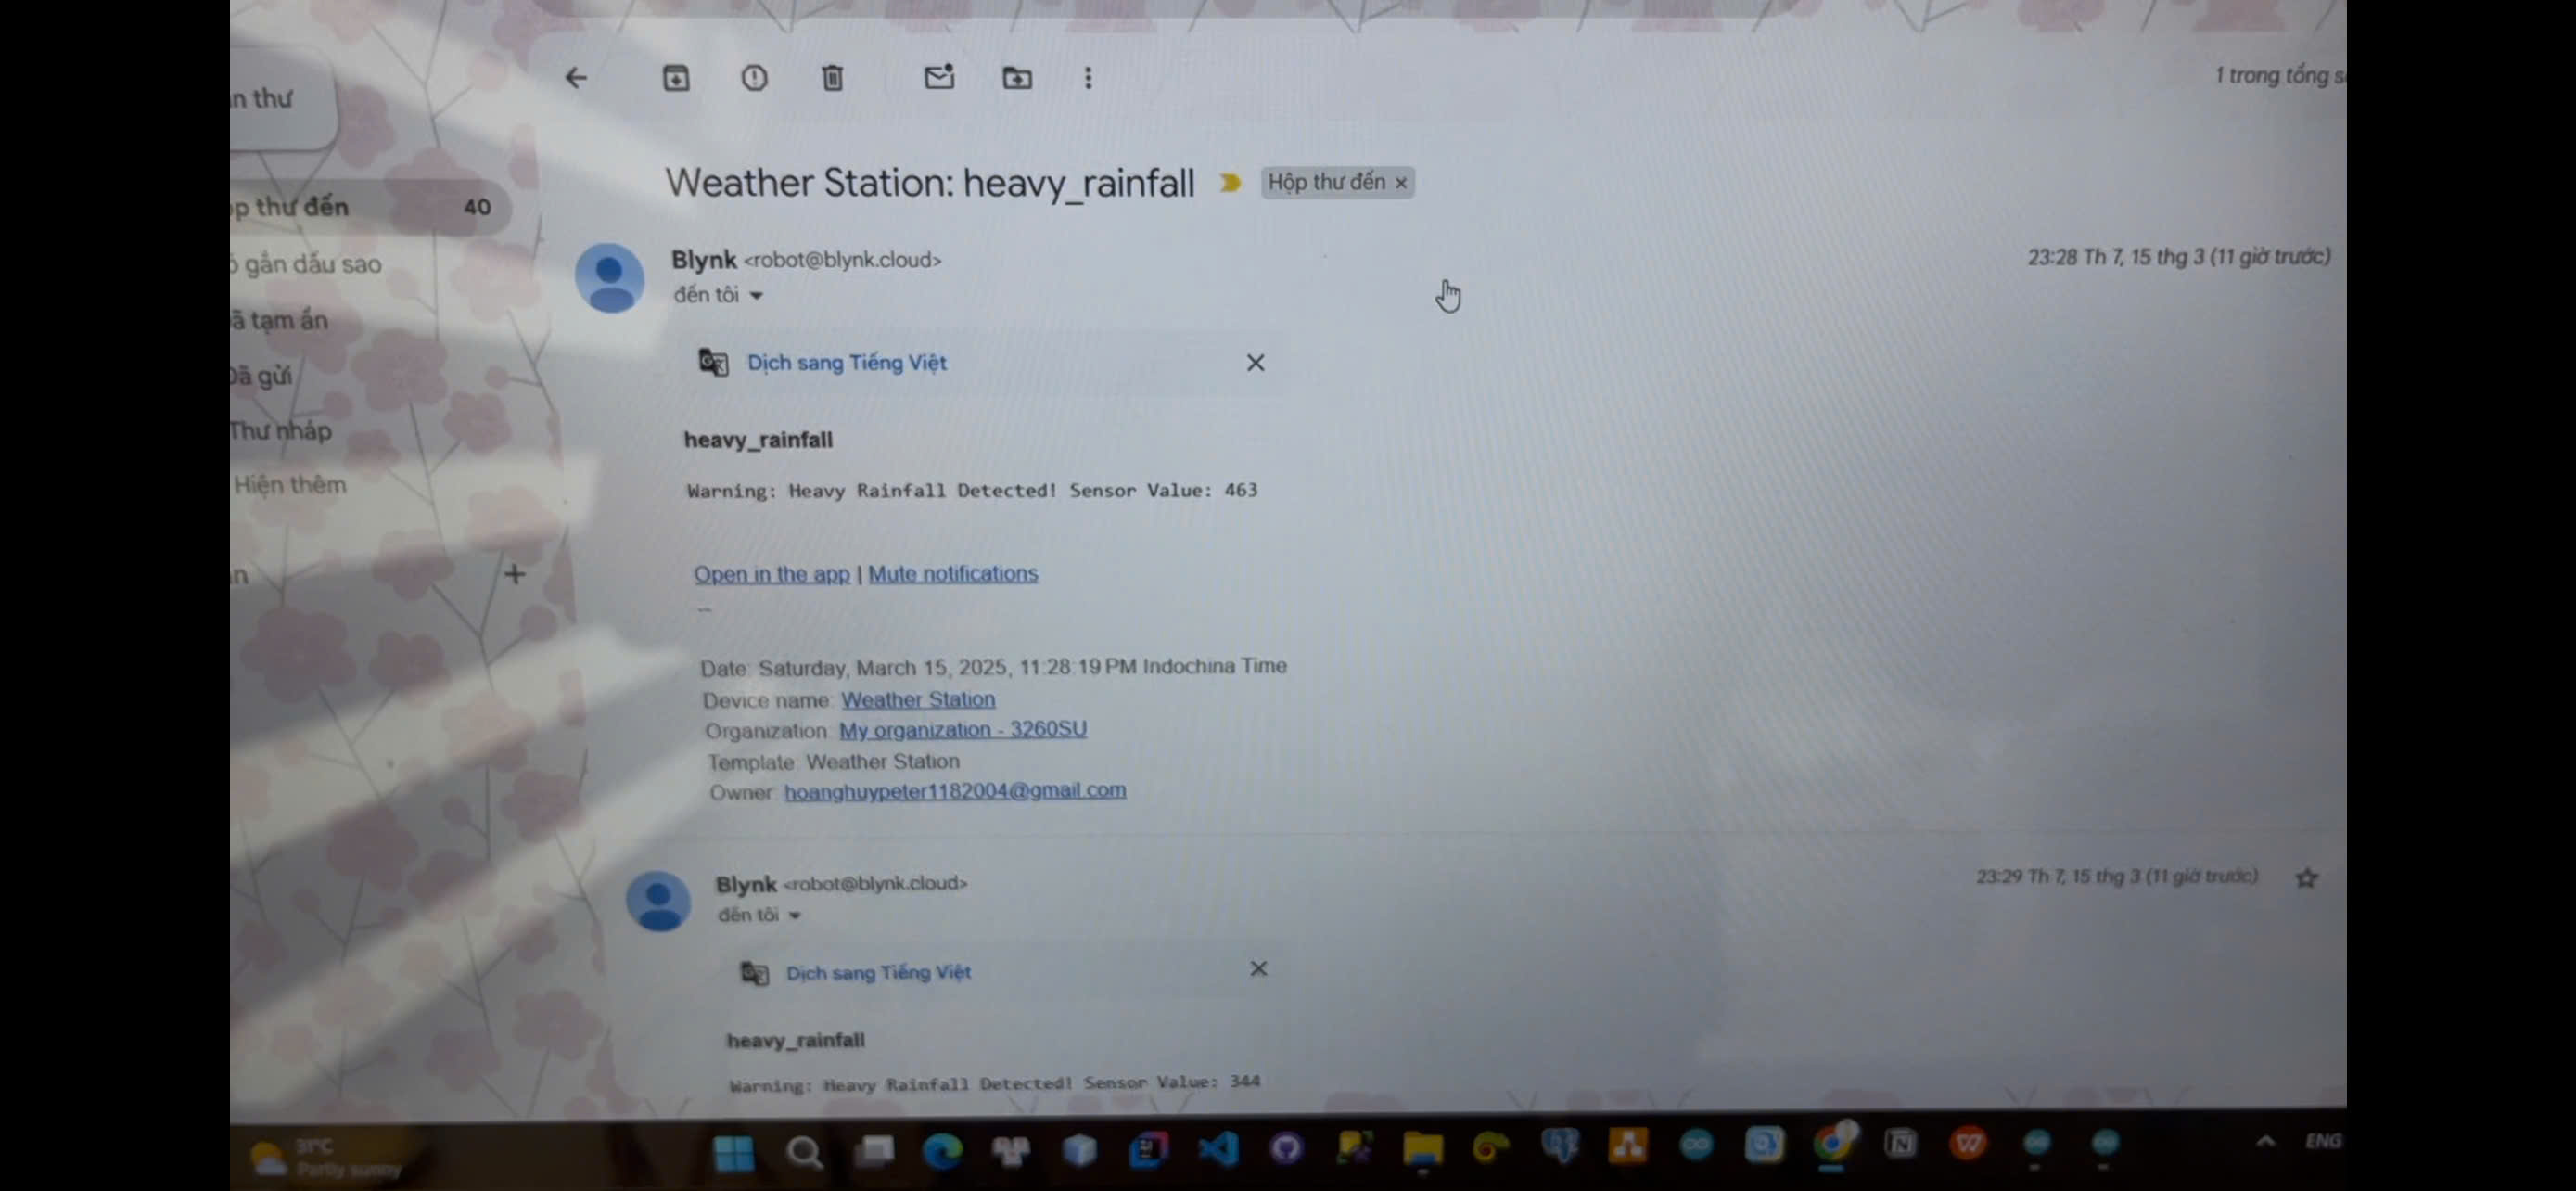
\includegraphics[width=0.9\linewidth]{figures/z6411778633153_203678abd880ad2fa383207659a97fd6.jpg}
        \caption{Notifications via Email}
        \label{fig:email_notifications}
    \end{subfigure}
    \begin{subfigure}{0.45\textwidth}
        \centering
        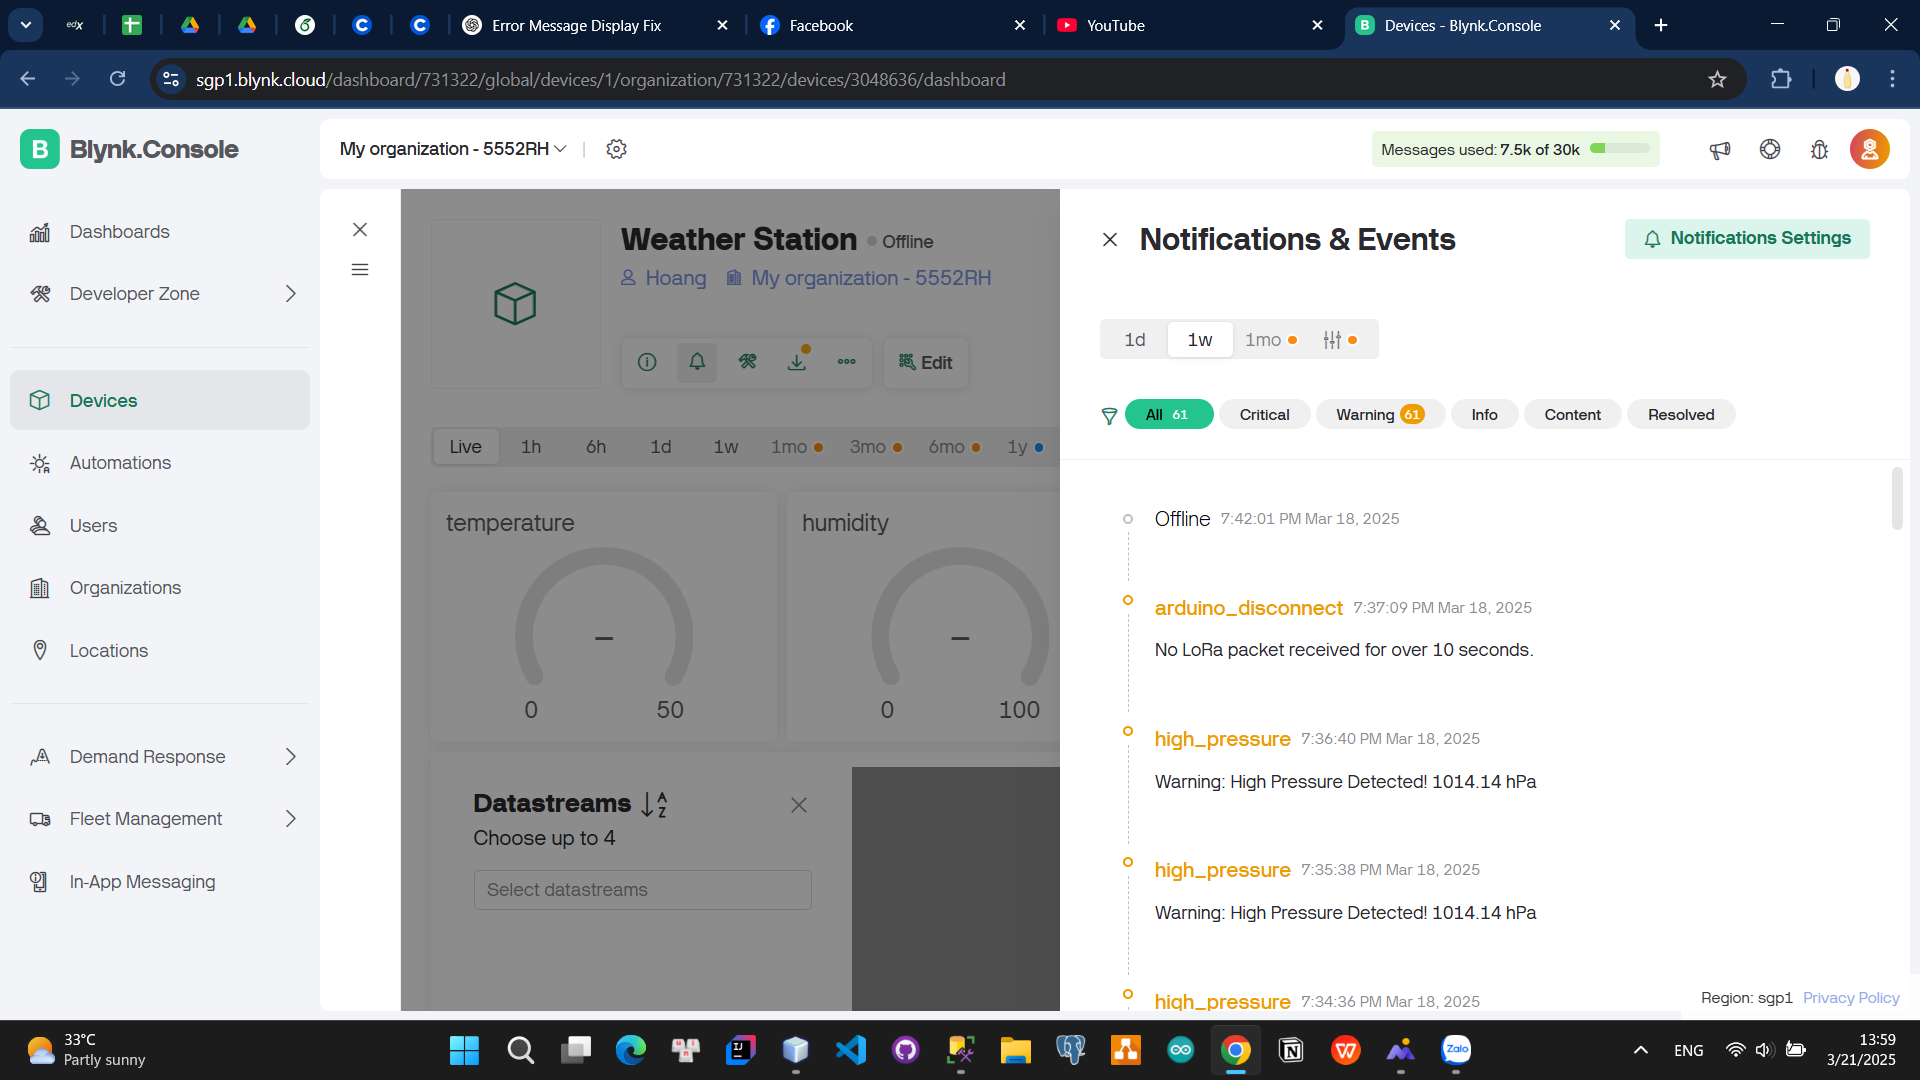
\includegraphics[width=0.9\linewidth]{figures/Screenshot (207).png}
        \caption{Alerts on Blynk Web}
        \label{fig:web_alerts}
    \end{subfigure}
    \caption{Alerts and Notifcations displayed via Blynk App and Email}
    \label{fig:alerts_and_notifications}
\end{figure}

\subsection{Discussion}
\subsubsection{\textbf{Key achievements}}
\begin{itemize}
    \item Accurate Data Collection: The system correctly measured temperature, humidity, pressure, and rain.
    \item Wireless Data Transfer: LoRa and WiFi-based communication enabled remote access to meteorological data.
    \item Real-Time Monitoring and Alerts: The Blynk app displayed live data and sent alerts for extreme weather conditions.
\end{itemize}

\subsubsection{\textbf{Challenges}}
\begin{itemize}
    \item Sensor Accuracy and Calibration: Low-cost sensors like DHT11 and BMP180 are not highly accurate and may require multiple calibrations at times to provide correct data.
    \item WiFi Connectivity Problems: The ESP8266 NodeMCU relies on reliable WiFi networks; poor signals or network loss will lead to data loss or delayed data transmission.
    \item Data Storage Limitations: Free Blynk cloud services usually have limited storage space, requiring periodic data management (every 30 days) or a shift to paid services.
    \item Security Threats: Since the system sends data through WiFi and LoRa, it is vulnerable to hacking, unauthorized access, or data leaks if not secured.
\end{itemize}

\subsubsection{\textbf{Future works}}
\begin{itemize}
    \item Integration of Additional Sensors:
        \begin{itemize}
            \item Air Quality Sensor (MQ135): Monitor pollution levels for environmental monitoring.
            \item UV and Solar Radiation Sensors: Expand climate study applications.
        \end{itemize}
    \item Improved power management through solar panel and battery backup enables round-the-clock operation, making the system independent in remote areas.
    \item Advanced Data Visualization and Storage: Google Firebase integration can store weather data for future analysis over a long period of time.
    \item Securing Communication and Cloud Data: Implementing AES Encryption for LoRa data transmission can protect sensor data from being used without authorization.
\end{itemize}

\vspace{10pt}
\noindent\rule{\textwidth}{0.4pt}
\vspace{10pt}

%----------------- Section IV: Conclusion -----------------
\section{CONCLUSION}
The weather station project achieved various milestones, including the capture of reliable data, data transmission wirelessly, and observation in real-time with alerts. Despite these successes, the project had challenges like sensor accuracy issues, WiFi connectivity issues, data storage limitations, and security threats. In the future, the project is planned to include the integration of additional sensors, including air quality sensor (MQ135), and solar radiation and UV sensors, together with more robust power management in the form of solar panels and battery backup. Software and cloud upgrades are also being contemplated involving platforms such as Google Firebase and implementing AES encryption for transmitting data using LoRa in a bid to secure data in the cloud and communication. Overall, this project has laid a strong foundation for future research in environmental monitoring by bringing to the fore such key challenges and opportunities, and it is bound to result in tremendous advancements in weather forecasting and related research.

\vspace{10pt}
\noindent\rule{\textwidth}{0.4pt}
\vspace{10pt}

%----------------- Section V: Author's Contribution -----------------
\section{AUTHOR'S CONTRIBUTION}

\begin{table}[H]
    \centering
    \begin{tabular}{|c|c|c|p{5cm}|c|}
    \hline
         \# & Student ID & Student Name & Tasks & Contribution \\
    \hline
         1 & SE184005 & Tran Dinh Son & Project Planning and Documentation \newline Testing, Experimentation, and Data Analysis & 22\% \\
    \hline
         2 & SE192052 & Truong Le Huy Hoang & Project Planning and Documentation \newline Hardware Design and Assembly \newline Software Development and Programming & 34\% \\
    \hline
         3 & SE182173 & Nguyen Binh Minh & Project Planning and Documentation \newline Visualization and Presentation & 22\% \\
    \hline
         4 & SE182141 & Vo Nhat Thien & Project Planning and Documentation \newline Visualization and Presentation & 22\% \\
    \hline
         \multicolumn{4}{|c|}{Total} & 100\% \\
    \hline
    \end{tabular}
    \label{tab:task_distribution}
\end{table}

\vspace{10pt}
\noindent\rule{\textwidth}{0.4pt}
\vspace{10pt}

\bibliographystyle{IEEEtran}
\bibliography{Bib_references}
\cite{Rahman2020,Guo2020,Singh2019,Zhang2021,Ahmed2018}

\end{document}
